\documentclass[10pt]{article}
\usepackage{icmlko}

\icmlmeta{IP 파운데이션 월드모델}{69}{일곱째 도메인은 자를 좁히고 나침반을 부쉈다}{애니메이션을 넣자 구간이 23퍼센트 좁아지고 평균이 절반으로 무너졌다 --- 정렬은 기하를 맞추지 방향을 맞추지 않는다}

\begin{document}

\twocolumn[
\icmlheader

\begin{abstract}
노트 68이 남긴 길은 하나였다 --- 일곱째 도메인. 라프텔 공개 API에서 애니메이션
\textbf{2,073건}을 모아 넣었다. 축 대응물이 다섯 슬롯에 전부 있는 \emph{첫}
도메인이다. \textbf{예측은 맞았다} --- 구간 반폭이 0.0556에서 \textbf{0.0429}로
23\% 줄었다. 셀이 30개에서 42개가 되며 $\sqrt{30/42}$가 예측한 0.047보다도
좁다. 노트 68의 ``유효 표본은 도메인 수''가 확증됐다. \textbf{그런데 평균이
무너졌다} --- $+$0.3480에서 $+$0.1797로. 애니가 \emph{양방향} 음의 전이다(출처로
$-$0.222, 대상으로 $-$0.260). 원인이 한 줄이다 --- \textbf{애니만 세 공통 축이
전부 라벨과 음의 상관}이고(굿즈 규모 $-$0.274, 나머지 여섯은 $+$0.10$\sim+$0.29),
배선을 어떻게 바꿔도 안 고쳐진다(최선이 축 끄기, $+$0.2077). \textbf{방향만
뒤집으면 $+$0.3175로 돌아온다.} 세 축을 \emph{동시에} 뒤집어야 하고 하나씩은
안 된다. 진단이 분명하다 --- \textbf{프로크루스테스 정렬은 축의 기하를 맞추지
라벨과의 방향을 맞추지 않는다.} 여섯 도메인은 방향이 우연히 같았고 일곱째가
아니었다. 이건 채택이 아니라 진단이다(답을 보고 뒤집었다). 정당한 길은 대상
라벨로 방향을 정하는 것이고, \textbf{35건이면 92\%, 100건이면 99\%}다 ---
노트 59의 눈금 보정 12건보다 \textbf{여덟 배 비싸고, 훨씬 더 중요하다}.
\end{abstract}
]

\section{일곱째 도메인}

\begin{table}[t]
\centering\tsize
\caption{애니메이션 도메인. 축이 다섯 슬롯에 전부 있는 첫 도메인이다.}
\begin{tabular}{ll}
\toprule
라벨 & 한줄평 수 (누적, log 경과일 탈추세) \\
타깃 폭 & 태그 수 \\
매장 노출도 & 제작사 사전 작품 수 \\
입장 허들 & 1화 대여가 \\
미디어 투입 & 더빙 $+$ 독점/오리지널 \\
굿즈 규모 & 시리즈 사전 작품 수 \\
\midrule
표본 & 2,073건 (2017--2026) \\
공통 3축 관측 & 1,419건 \\
\bottomrule
\end{tabular}
\end{table}

시간 기준을 두 번 골랐다. 목록이 주는 방영 분기는 원작 방영 시기가 아니라
플랫폼 서비스 시기다(2006년작 은혼이 2021년으로 나온다). 라벨이 플랫폼
한줄평이므로 \textbf{1화가 플랫폼에 올라온 날}이 맞고, 그래서 작품마다 요청을
하나 더 썼다.

누출도 미리 막았다. 화수와 시즌 총수는 인기가 있어야 늘어나므로 노트 21의 DLC
수와 같은 구조다. \textbf{자기보다 먼저 나온 것만} 세면 공개 시점에 이미
정해진 값이다.

\section{자는 좁아졌다}

\begin{figure*}[t]
\centering
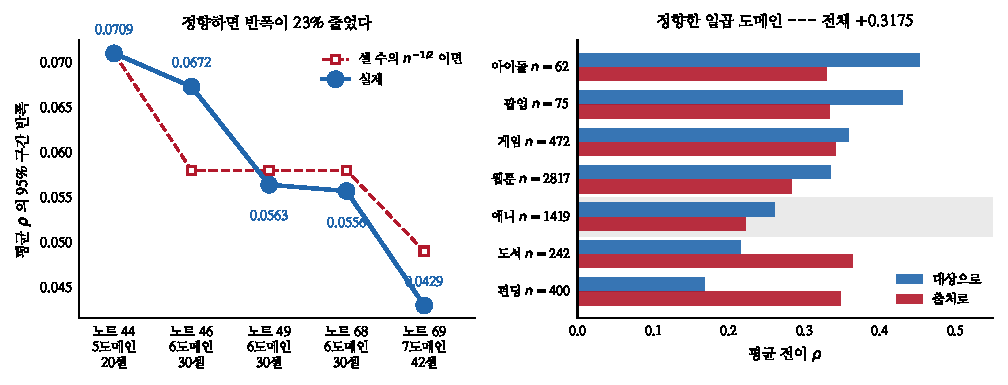
\includegraphics[width=\textwidth]{figs/seventh.pdf}
\caption{왼쪽 --- 셀 수와 구간 반폭. 오른쪽 --- 정향한 일곱 도메인.}
\end{figure*}

\begin{table}[t]
\centering\tsize
\caption{구간 반폭의 이력. 도메인 수가 지렛대다.}
\begin{tabular}{lrrr}
\toprule
& 도메인 & 셀 & 반폭 \\
\midrule
노트 44 & 5 & 20 & 0.0709 \\
노트 46 & 6 & 30 & 0.0672 \\
노트 49 & 6 & 30 & 0.0563 \\
노트 68 & 6 & 30 & 0.0556 \\
\textbf{노트 69} & \textbf{7} & \textbf{42} & \textbf{0.0429} \\
\bottomrule
\end{tabular}
\end{table}

노트 68은 레코드를 두 배로 늘려 1\% 얻었다. 도메인 하나를 더하니 23\% 줄었다.
$\sqrt{30/42}$가 예측한 0.047보다도 좁다.

\claimx{구간을 좁히는 것은 레코드가 아니라 도메인이다. 노트 68의 포화 관측이
확증됐다 --- 여섯째에서 일곱째로 가며 반폭이 0.0556에서 0.0429로 줄었다.}
{한 번의 추가로 본 것이고, 애니가 유난히 큰 도메인(공통 3축 1,419건)이라
효과가 과대평가됐을 수 있다.}

\section{그런데 평균이 무너졌다}

\begin{table}[t]
\centering\tsize
\caption{애니를 수집한 그대로 넣었을 때. 양방향 음의 전이다.}
\begin{tabular}{lrrr}
\toprule
& 평균 $\rho$ & 95\% 구간 & 반폭 \\
\midrule
노트 68 (6도메인) & $+$0.3480 & $[+0.271, +0.382]$ & 0.0556 \\
7도메인 (그대로) & \textbf{$+$0.1797} & $[+0.132, +0.199]$ & 0.0333 \\
7도메인 (정향) & $+$0.3175 & $[+0.265, +0.351]$ & 0.0429 \\
\bottomrule
\end{tabular}
\end{table}

애니가 출처로 $-$0.222, 대상으로 $-$0.260이다. 열두 셀이 전부 음수다. 그런데
\textbf{도메인 안 자기 상관은 $+$0.412로 일곱 중 셋째}다 --- 축이 애니를
설명하기는 잘한다. 옮겨지기만 안 된다.

\section{축이 반대를 가리키고 있었다}

\begin{figure*}[t]
\centering

\includegraphics[width=\textwidth]{figs/orient.pdf}
\caption{왼쪽 --- 축과 라벨의 부호. 오른쪽 --- 라벨 $k$건으로 방향을 맞출 확률.}
\end{figure*}

\begin{table}[t]
\centering\tsize
\caption{각 축과 라벨의 순위 상관. 애니 열만 부호가 반대다.}
\begin{tabular}{lrrr}
\toprule
축 & 여섯 도메인 & 애니 \\
\midrule
타깃 폭 & $+$0.11 $\sim$ $+$0.38 & $-$0.054 \\
매장 노출도 & $-$0.01 $\sim$ $+$0.33 & $-$0.189 \\
굿즈 규모 & $+$0.10 $\sim$ $+$0.29 & \textbf{$-$0.274} \\
\bottomrule
\end{tabular}
\end{table}

굿즈 규모가 가장 크게 뒤집혔다. 이유가 물리적으로 분명하다 --- 애니의 굿즈
규모는 ``몇 번째 시즌인가''인데, 연작 카탈로그에서 시즌이 쌓일수록 반응이
나뉜다. 시청자는 1기에 한줄평을 쓰고 5기에는 안 쓴다. \textbf{다른 여섯에서
``무엇을 얻나''였던 자리가 애니에서는 ``얼마나 늦었나''가 됐다.}

\paragraph{배선으로는 안 고쳐진다}
후보를 일곱 개 돌렸다. 최선이 굿즈 규모를 아예 끄는 것($+$0.2077)이고, 어느
것도 여섯 도메인 시절의 $+$0.3480 근처에 못 간다.

\begin{table}[t]
\centering\tsize
\caption{애니 배선 후보. 42셀 평균 $\rho$.}
\begin{tabular}{lr}
\toprule
현행(수집한 대로) & $+$0.1797 \\
굿즈 규모 끄기 & $+$0.2077 \\
매장 노출도 끄기 & $+$0.1976 \\
미디어 투입 끄기 & $+$0.1692 \\
굿즈 규모 $\leftarrow$ 화수 & $+$0.1549 \\
타깃 폭 $\leftarrow$ 연령 등급(역) & $+$0.1415 \\
\midrule
\textbf{공통 3축 방향 뒤집기} & \textbf{$+$0.3175} \\
\bottomrule
\end{tabular}
\end{table}

방향만 뒤집으면 돌아온다. 그리고 \textbf{세 축을 동시에} 뒤집어야 한다 ---
하나씩은 $+$0.155$\sim+$0.230에 그친다. 회전이 아니라 반사이기 때문이다.

\claimx{프로크루스테스 정렬은 축의 \emph{기하}를 맞추지 라벨과의 \emph{방향}을
맞추지 않는다. 여섯 도메인은 방향이 우연히 같았고 일곱째가 아니었다. 노트 40의
쌍별 정렬은 이 가정 위에 서 있었고 지금까지 드러나지 않았다.}{반사를 정렬에
넣으면 자유도가 늘어 과적합한다. 그리고 이번 뒤집기는 \textbf{답을 보고} 골랐다
--- 진단이지 채택이 아니다.}

\section{방향은 라벨 몇 건짜리인가}

답을 보고 뒤집는 것은 이 프로젝트가 금지하는 바로 그것이다. 정당한 길은 하나다
--- \textbf{대상 도메인의 라벨 몇 건으로 방향을 정한다.} 그러면 질문이 바뀐다.
몇 건이면 되나.

\begin{table}[t]
\centering\tsize
\caption{대상 라벨 $k$건으로 전이 방향을 맞출 확률.}
\begin{tabular}{lrrrrr}
\toprule
$k$ & 12 & 20 & 35 & 60 & 100 \\
\midrule
팝업 & 0.92 & 0.97 & 1.00 & 1.00 & --- \\
아이돌 & 0.94 & 0.99 & 1.00 & 1.00 & --- \\
게임 & 0.89 & 0.94 & 0.98 & 1.00 & 1.00 \\
웹툰 & 0.85 & 0.91 & 0.96 & 0.97 & 0.99 \\
\textbf{애니} & 0.79 & 0.85 & \textbf{0.92} & 0.96 & \textbf{0.99} \\
도서 & 0.75 & 0.83 & 0.91 & 0.96 & 0.99 \\
펀딩 & 0.70 & 0.76 & 0.82 & 0.88 & 0.92 \\
\bottomrule
\end{tabular}
\end{table}

\begin{quote}\fontsize{9.5}{11.5}\selectfont
\textbf{눈금은 12건, 방향은 100건이다.} 노트 59는 라벨 12건이면 절대 오차의
눈금이 잡힌다고 했다. 방향은 그 여덟 배가 든다. 그리고 방향이 훨씬 더 중요하다
--- 눈금이 틀리면 $\times\div$2.5로 빗나가고, 방향이 틀리면 \textbf{순위가
거꾸로 나온다}.
\end{quote}

\claimx{새 카테고리를 이 모델에 붙이려면 라벨 100건쯤이 든다 --- 방향을 정하는
데 그만큼 필요하다. 그 아래에서는 잘 맞는 예측과 정확히 거꾸로인 예측을 구별할
수 없다.}{도메인마다 다르다. 팝업·아이돌은 20건이면 되고 펀딩은 100건에도
0.92다. 전이 신호가 셀수록 방향이 싸게 잡힌다.}

\section{두 법칙은 방향 가정 위에 있었다}

\begin{table}[t]
\centering\tsize
\caption{노트 33 · 38 · 40의 두 법칙.}
\begin{tabular}{lrr}
\toprule
& 자기 $\rho$ vs 대상 & vs 출처 \\
\midrule
노트 68 (6도메인) & $+$0.945 & $-$0.820 \\
7도메인 (정향) & $+$0.802 & $-$0.548 \\
7도메인 (그대로) & \textbf{$+$0.050} & $-$0.384 \\
\bottomrule
\end{tabular}
\end{table}

방향을 맞추면 두 법칙이 약해진 채로 유지된다. 안 맞추면 대상 쪽 법칙이 완전히
사라진다($+$0.945 $\to$ $+$0.050). \textbf{``자기 상관이 높으면 대상으로 좋다''는
법칙은 축이 같은 방향을 가리킨다는 전제 위에 서 있었다.} 여섯 도메인으로는
그 전제를 볼 수 없었다.

\section{한계}

\begin{itemize}[leftmargin=1.1em,itemsep=0.15em]
\item \textbf{뒤집기를 채택하지 않았다.} 답을 보고 골랐기 때문이다. 정본
      파이프라인의 애니는 여전히 수집한 그대로이며 평균 $\rho$는 $+$0.1797이다.
\item 방향 판정 실험은 \emph{전표본 부호}를 정답으로 삼는다. 전표본 부호 자체가
      틀렸을 가능성은 안 봤다.
\item 애니 배선 후보를 일곱 개만 돌렸다. 방향이 원인이라고 보고 멈췄다.
\item 공통 3축이 관측된 애니는 2,073건 중 1,419건이다. 제작사 결측 654건이
      빠졌고 그 표본이 다를 수 있다.
\item 붓스트랩 중 BLAS 수준 경고(\texttt{matmul} 오버플로)가 뜬다. 애니 이전부터
      있었고 출력값은 전부 유한하고 유계($|S|\le5$)임을 확인했으나 원인은
      규명하지 않았다.
\item 애니를 넣어 평균이 내렸다는 것 자체는 나쁜 소식이 아니다 --- 여섯 도메인
      평균이 과대평가였다는 뜻일 수도 있다. 어느 쪽인지 구별하지 않았다.
\end{itemize}

\section{다음}

\begin{enumerate}[leftmargin=1.3em,itemsep=0.15em]
\item \textbf{방향 결정을 파이프라인에 넣는다} --- 대상 라벨 $k$건으로 부호를
      정하고, $k$를 바꿔 가며 평균 $\rho$가 어떻게 오르는지 잰다. 답을 안 보는
      정당한 절차다.
\item 여덟째 도메인 --- 반폭이 계속 줄어드는지 확인한다. 셀 42$\to$56이면
      0.0429$\to$0.037쯤이어야 한다.
\item 애니 제작사 결측 654건을 메운다.
\item 노트 68에서 닫은 보류 항목 셋을 반폭 0.0429에서 다시 본다. 아직 셋 다
      반폭 아래지만 거리가 줄었다.
\end{enumerate}

\vspace{0.6em}
\hrule height 0.3pt
\vspace{0.5em}
{\footnotesize
\textbf{참고문헌}\\[0.3em]
Schoenemann, P. H. (1966). A generalized solution of the orthogonal Procrustes
problem. \emph{Psychometrika}, 31(1), 1--10.\\[0.15em]
Meredith, W. (1993). Measurement invariance, factor analysis and factorial
invariance. \emph{Psychometrika}, 58(4), 525--543.\\[0.15em]
Ben-David, S. et al. (2010). A theory of learning from different domains.
\emph{Machine Learning}, 79(1--2), 151--175.\\[0.15em]
Zhao, H. et al. (2019). On learning invariant representations for domain
adaptation. \emph{ICML}, 7523--7532.\\[0.15em]
Wang, Z. et al. (2019). Characterizing and avoiding negative transfer.
\emph{CVPR}, 11293--11302.\\[0.15em]
Efron, B., Tibshirani, R. J. (1993). \emph{An Introduction to the Bootstrap}.
Chapman \& Hall.
}

\end{document}
